% Options for packages loaded elsewhere
% Options for packages loaded elsewhere
\PassOptionsToPackage{unicode}{hyperref}
\PassOptionsToPackage{hyphens}{url}
\PassOptionsToPackage{dvipsnames,svgnames,x11names}{xcolor}
%
\documentclass[
  letterpaper,
  DIV=11,
  numbers=noendperiod]{scrartcl}
\usepackage{xcolor}
\usepackage[margin=1in]{geometry}
\usepackage{amsmath,amssymb}
\setcounter{secnumdepth}{5}
\usepackage{iftex}
\ifPDFTeX
  \usepackage[T1]{fontenc}
  \usepackage[utf8]{inputenc}
  \usepackage{textcomp} % provide euro and other symbols
\else % if luatex or xetex
  \usepackage{unicode-math} % this also loads fontspec
  \defaultfontfeatures{Scale=MatchLowercase}
  \defaultfontfeatures[\rmfamily]{Ligatures=TeX,Scale=1}
\fi
\usepackage{lmodern}
\ifPDFTeX\else
  % xetex/luatex font selection
\fi
% Use upquote if available, for straight quotes in verbatim environments
\IfFileExists{upquote.sty}{\usepackage{upquote}}{}
\IfFileExists{microtype.sty}{% use microtype if available
  \usepackage[]{microtype}
  \UseMicrotypeSet[protrusion]{basicmath} % disable protrusion for tt fonts
}{}
\makeatletter
\@ifundefined{KOMAClassName}{% if non-KOMA class
  \IfFileExists{parskip.sty}{%
    \usepackage{parskip}
  }{% else
    \setlength{\parindent}{0pt}
    \setlength{\parskip}{6pt plus 2pt minus 1pt}}
}{% if KOMA class
  \KOMAoptions{parskip=half}}
\makeatother
% Make \paragraph and \subparagraph free-standing
\makeatletter
\ifx\paragraph\undefined\else
  \let\oldparagraph\paragraph
  \renewcommand{\paragraph}{
    \@ifstar
      \xxxParagraphStar
      \xxxParagraphNoStar
  }
  \newcommand{\xxxParagraphStar}[1]{\oldparagraph*{#1}\mbox{}}
  \newcommand{\xxxParagraphNoStar}[1]{\oldparagraph{#1}\mbox{}}
\fi
\ifx\subparagraph\undefined\else
  \let\oldsubparagraph\subparagraph
  \renewcommand{\subparagraph}{
    \@ifstar
      \xxxSubParagraphStar
      \xxxSubParagraphNoStar
  }
  \newcommand{\xxxSubParagraphStar}[1]{\oldsubparagraph*{#1}\mbox{}}
  \newcommand{\xxxSubParagraphNoStar}[1]{\oldsubparagraph{#1}\mbox{}}
\fi
\makeatother

\usepackage{color}
\usepackage{fancyvrb}
\newcommand{\VerbBar}{|}
\newcommand{\VERB}{\Verb[commandchars=\\\{\}]}
\DefineVerbatimEnvironment{Highlighting}{Verbatim}{commandchars=\\\{\}}
% Add ',fontsize=\small' for more characters per line
\usepackage{framed}
\definecolor{shadecolor}{RGB}{241,243,245}
\newenvironment{Shaded}{\begin{snugshade}}{\end{snugshade}}
\newcommand{\AlertTok}[1]{\textcolor[rgb]{0.68,0.00,0.00}{#1}}
\newcommand{\AnnotationTok}[1]{\textcolor[rgb]{0.37,0.37,0.37}{#1}}
\newcommand{\AttributeTok}[1]{\textcolor[rgb]{0.40,0.45,0.13}{#1}}
\newcommand{\BaseNTok}[1]{\textcolor[rgb]{0.68,0.00,0.00}{#1}}
\newcommand{\BuiltInTok}[1]{\textcolor[rgb]{0.00,0.23,0.31}{#1}}
\newcommand{\CharTok}[1]{\textcolor[rgb]{0.13,0.47,0.30}{#1}}
\newcommand{\CommentTok}[1]{\textcolor[rgb]{0.37,0.37,0.37}{#1}}
\newcommand{\CommentVarTok}[1]{\textcolor[rgb]{0.37,0.37,0.37}{\textit{#1}}}
\newcommand{\ConstantTok}[1]{\textcolor[rgb]{0.56,0.35,0.01}{#1}}
\newcommand{\ControlFlowTok}[1]{\textcolor[rgb]{0.00,0.23,0.31}{\textbf{#1}}}
\newcommand{\DataTypeTok}[1]{\textcolor[rgb]{0.68,0.00,0.00}{#1}}
\newcommand{\DecValTok}[1]{\textcolor[rgb]{0.68,0.00,0.00}{#1}}
\newcommand{\DocumentationTok}[1]{\textcolor[rgb]{0.37,0.37,0.37}{\textit{#1}}}
\newcommand{\ErrorTok}[1]{\textcolor[rgb]{0.68,0.00,0.00}{#1}}
\newcommand{\ExtensionTok}[1]{\textcolor[rgb]{0.00,0.23,0.31}{#1}}
\newcommand{\FloatTok}[1]{\textcolor[rgb]{0.68,0.00,0.00}{#1}}
\newcommand{\FunctionTok}[1]{\textcolor[rgb]{0.28,0.35,0.67}{#1}}
\newcommand{\ImportTok}[1]{\textcolor[rgb]{0.00,0.46,0.62}{#1}}
\newcommand{\InformationTok}[1]{\textcolor[rgb]{0.37,0.37,0.37}{#1}}
\newcommand{\KeywordTok}[1]{\textcolor[rgb]{0.00,0.23,0.31}{\textbf{#1}}}
\newcommand{\NormalTok}[1]{\textcolor[rgb]{0.00,0.23,0.31}{#1}}
\newcommand{\OperatorTok}[1]{\textcolor[rgb]{0.37,0.37,0.37}{#1}}
\newcommand{\OtherTok}[1]{\textcolor[rgb]{0.00,0.23,0.31}{#1}}
\newcommand{\PreprocessorTok}[1]{\textcolor[rgb]{0.68,0.00,0.00}{#1}}
\newcommand{\RegionMarkerTok}[1]{\textcolor[rgb]{0.00,0.23,0.31}{#1}}
\newcommand{\SpecialCharTok}[1]{\textcolor[rgb]{0.37,0.37,0.37}{#1}}
\newcommand{\SpecialStringTok}[1]{\textcolor[rgb]{0.13,0.47,0.30}{#1}}
\newcommand{\StringTok}[1]{\textcolor[rgb]{0.13,0.47,0.30}{#1}}
\newcommand{\VariableTok}[1]{\textcolor[rgb]{0.07,0.07,0.07}{#1}}
\newcommand{\VerbatimStringTok}[1]{\textcolor[rgb]{0.13,0.47,0.30}{#1}}
\newcommand{\WarningTok}[1]{\textcolor[rgb]{0.37,0.37,0.37}{\textit{#1}}}

\usepackage{longtable,booktabs,array}
\usepackage{calc} % for calculating minipage widths
% Correct order of tables after \paragraph or \subparagraph
\usepackage{etoolbox}
\makeatletter
\patchcmd\longtable{\par}{\if@noskipsec\mbox{}\fi\par}{}{}
\makeatother
% Allow footnotes in longtable head/foot
\IfFileExists{footnotehyper.sty}{\usepackage{footnotehyper}}{\usepackage{footnote}}
\makesavenoteenv{longtable}
\usepackage{graphicx}
\makeatletter
\newsavebox\pandoc@box
\newcommand*\pandocbounded[1]{% scales image to fit in text height/width
  \sbox\pandoc@box{#1}%
  \Gscale@div\@tempa{\textheight}{\dimexpr\ht\pandoc@box+\dp\pandoc@box\relax}%
  \Gscale@div\@tempb{\linewidth}{\wd\pandoc@box}%
  \ifdim\@tempb\p@<\@tempa\p@\let\@tempa\@tempb\fi% select the smaller of both
  \ifdim\@tempa\p@<\p@\scalebox{\@tempa}{\usebox\pandoc@box}%
  \else\usebox{\pandoc@box}%
  \fi%
}
% Set default figure placement to htbp
\def\fps@figure{htbp}
\makeatother





\setlength{\emergencystretch}{3em} % prevent overfull lines

\providecommand{\tightlist}{%
  \setlength{\itemsep}{0pt}\setlength{\parskip}{0pt}}



 


\usepackage{float}
\usepackage{tabularray}
\usepackage[normalem]{ulem}
\usepackage{graphicx}
\usepackage{rotating}
\UseTblrLibrary{siunitx}
\NewTableCommand{\tinytableDefineColor}[3]{\definecolor{#1}{#2}{#3}}
\newcommand{\tinytableTabularrayUnderline}[1]{\underline{#1}}
\newcommand{\tinytableTabularrayStrikeout}[1]{\sout{#1}}
\KOMAoption{captions}{tableheading}
\makeatletter
\@ifpackageloaded{caption}{}{\usepackage{caption}}
\AtBeginDocument{%
\ifdefined\contentsname
  \renewcommand*\contentsname{Table of contents}
\else
  \newcommand\contentsname{Table of contents}
\fi
\ifdefined\listfigurename
  \renewcommand*\listfigurename{List of Figures}
\else
  \newcommand\listfigurename{List of Figures}
\fi
\ifdefined\listtablename
  \renewcommand*\listtablename{List of Tables}
\else
  \newcommand\listtablename{List of Tables}
\fi
\ifdefined\figurename
  \renewcommand*\figurename{Figure}
\else
  \newcommand\figurename{Figure}
\fi
\ifdefined\tablename
  \renewcommand*\tablename{Table}
\else
  \newcommand\tablename{Table}
\fi
}
\@ifpackageloaded{float}{}{\usepackage{float}}
\floatstyle{ruled}
\@ifundefined{c@chapter}{\newfloat{codelisting}{h}{lop}}{\newfloat{codelisting}{h}{lop}[chapter]}
\floatname{codelisting}{Listing}
\newcommand*\listoflistings{\listof{codelisting}{List of Listings}}
\makeatother
\makeatletter
\makeatother
\makeatletter
\@ifpackageloaded{caption}{}{\usepackage{caption}}
\@ifpackageloaded{subcaption}{}{\usepackage{subcaption}}
\makeatother
\usepackage{bookmark}
\IfFileExists{xurl.sty}{\usepackage{xurl}}{} % add URL line breaks if available
\urlstyle{same}
\hypersetup{
  pdftitle={Tell me who you are and i'll tell your position on the job market},
  pdfauthor={Varnel TIENTCHEU \& Shella LANKOANDE},
  colorlinks=true,
  linkcolor={blue},
  filecolor={Maroon},
  citecolor={Blue},
  urlcolor={Blue},
  pdfcreator={LaTeX via pandoc}}


\title{Tell me who you are and i'll tell your position on the job
market}
\author{Varnel TIENTCHEU \& Shella LANKOANDE}
\date{2026-04-13}
\begin{document}
\maketitle

\renewcommand*\contentsname{Table of contents}
{
\hypersetup{linkcolor=}
\setcounter{tocdepth}{3}
\tableofcontents
}

\begin{Shaded}
\begin{Highlighting}[]
\CommentTok{\# Installation des packages}
\FunctionTok{install.packages}\NormalTok{(}\StringTok{"haven"}\NormalTok{)}
\FunctionTok{install.packages}\NormalTok{(}\StringTok{"estimatr"}\NormalTok{)}
\FunctionTok{install.packages}\NormalTok{(}\StringTok{"tidyverse"}\NormalTok{)}
\FunctionTok{install.packages}\NormalTok{(}\StringTok{"fastDummies"}\NormalTok{)}
\FunctionTok{install.packages}\NormalTok{(}\StringTok{"corrplot"}\NormalTok{)}
\FunctionTok{install.packages}\NormalTok{(}\StringTok{"rstatix"}\NormalTok{)}
\FunctionTok{install.packages}\NormalTok{(}\StringTok{"modelsummary"}\NormalTok{)}
\FunctionTok{install.packages}\NormalTok{(}\StringTok{"plm"}\NormalTok{)}
\FunctionTok{install.packages}\NormalTok{(}\StringTok{"ggdag"}\NormalTok{)}
\CommentTok{\#{-}{-}{-}{-}{-}{-}{-}{-}{-}{-}{-}{-}{-}{-}{-}{-}{-}{-}{-}{-}{-}{-}{-}{-}{-}{-}{-}{-}{-}{-}{-}{-}{-}{-}{-}{-}{-}{-}{-}{-}{-}{-}{-}{-}{-}{-}{-}{-}{-}{-}{-}{-}{-}{-}{-}{-}{-}{-}{-}{-}{-}}
\FunctionTok{library}\NormalTok{(haven) }
\FunctionTok{library}\NormalTok{(plm)}
\FunctionTok{library}\NormalTok{(rstatix)}
\FunctionTok{library}\NormalTok{(estimatr)}
\FunctionTok{library}\NormalTok{(tidyverse)}
\FunctionTok{library}\NormalTok{(fastDummies)}
\FunctionTok{library}\NormalTok{(modelsummary)}
\FunctionTok{library}\NormalTok{(corrplot)}
\end{Highlighting}
\end{Shaded}

\section{I. Présentation du projet}\label{i.-pruxe9sentation-du-projet}

Ce projet vise à mesurer l'effet de différentes variables individuelles
sur la position sur le marché du travail, en particulier l'impact de
l'origine des individus sur le salaire horaire et le chômage.

Les données proviennent d'un panel de 10 000 individus suivis sur 6
trimestres (2014-2016).

Les principales variables sont\,:

\begin{itemize}
\tightlist
\item
  \textbf{Marge intensive} : salaire net horaire (\texttt{salhoraire},
  \texttt{logsalhoraire})
\item
  \textbf{Marge extensive} : statut sur le marché du travail (actif
  occupé, chômeur, inactif)
\item
  \textbf{Variables individuelles} : âge, sexe, diplôme, CSP des
  parents, origine, indicatrices immigré/descendant, état de santé,
  situation matrimoniale\ldots{}
\item
  \textbf{Variables géographiques} : région, tranche d'unité urbaine ,
  proportions de populations d'origines différentes\ldots{}
\end{itemize}

L'objectif est de déterminer si l'origine affecte le salaire et l'accès
à l'emploi, toutes choses égales par ailleurs.

Avant de passer à l'analyse économétrique, il est important de
s'approprier la base de données et de comprendre les caractéristiques
principales des individus suivis.

La base contient \textbf{10 000 individus} observés sur 6 trimestres
(2014-2016). On dispose d'informations sur les caractéristiques
individuelles (âge, sexe, diplôme, origine, état de santé, situation
matrimoniale), les caractéristiques professionnelles (statut sur le
marché du travail, salaire, heures travaillées, type de contrat) ainsi
que sur l'environnement géographique (région, tranche d'unité urbaine,
proportion de populations d'origines différentes).\\
Cette étape est essentielle pour \textbf{s'assurer de la qualité des
données}, guider le choix des variables explicatives et préparer
l'analyse économétrique qui suit.

\subsubsection{1) Chargement de la base de
données}\label{chargement-de-la-base-de-donnuxe9es}

Nous commençons par importer la base de données fournie pour le projet.

Le code suivant permet de lire le fichier \texttt{.dta} et de vérifier
ses dimensions (nombre de lignes et de colonnes) :

\begin{Shaded}
\begin{Highlighting}[]
\NormalTok{df }\OtherTok{\textless{}{-}} \FunctionTok{read\_dta}\NormalTok{(}\StringTok{"DM\_Subject\_2\_Data.dta"}\NormalTok{)}
\FunctionTok{dim}\NormalTok{(df)  }
\end{Highlighting}
\end{Shaded}

\begin{verbatim}
[1] 60000    60
\end{verbatim}

\begin{Shaded}
\begin{Highlighting}[]
\NormalTok{df}\SpecialCharTok{$}\NormalTok{salhoraire }\OtherTok{=}\NormalTok{ df}\SpecialCharTok{$}\NormalTok{salmensuel }\SpecialCharTok{/}\NormalTok{ (df}\SpecialCharTok{$}\NormalTok{heuretra }\SpecialCharTok{*} \FloatTok{4.33}\NormalTok{)}
\end{Highlighting}
\end{Shaded}

\subsubsection{2) Statistiques
descriptives}\label{statistiques-descriptives}

\pandocbounded{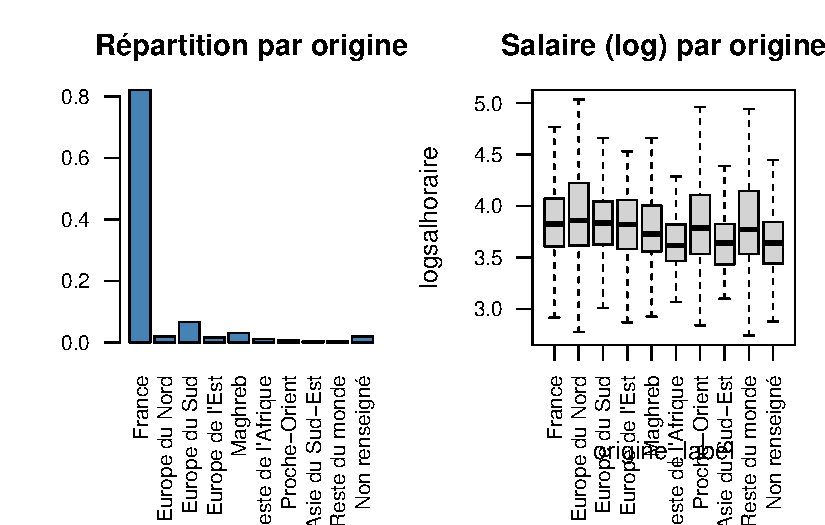
\includegraphics[keepaspectratio]{Rapport_files/figure-pdf/unnamed-chunk-3-1.pdf}}

\pandocbounded{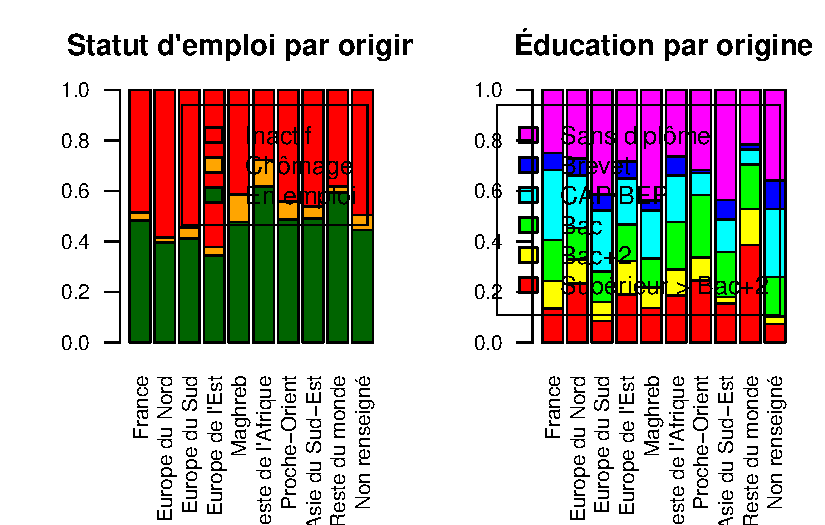
\includegraphics[keepaspectratio]{Rapport_files/figure-pdf/unnamed-chunk-3-2.pdf}}

L'échantillon est massivement dominé par l'origine française (plus de 80
\%). On observe une hétérogénéité marquée du capital humain : les
populations originaires du Maghreb et Asie du Sud-Est présentent une
part importante de non-diplômés, tandis que les origines d'Europe du
Nord ou du Reste du monde affichent des taux de diplômes supérieurs
élevés. Cette stratification éducative initiale confirme que le diplôme
est un canal de transmission majeur des inégalités salariales qu'il
faudra isoler.

Sur le marché du travail, les disparités sont visibles dès l'accès à
l'emploi (marge extensive) : les origines africaines et maghrébines
affichent des parts de chômage plus prononcées que la moyenne. Côté
salaires (marge intensive), si les médianes des logs-salaires semblent
globalement alignées, on distingue un tassement vers le bas pour le
Reste de l'Afrique et l'Asie du Sud-Est. La forte dispersion dans tous
les groupes, couplée à ces différences de médianes malgré des profils
éducatifs parfois élevés, justifie la problématique de recherche d'un
effet direct de l'origine au-delà des seules caractéristiques
productives.

\section{II. Marge Intensive}\label{ii.-marge-intensive}

Dans un premier temps, on étudie le salaire des actifs occupés et on
s'intéresse à l'existence de potentielles inégalités salariales dues à
l'origine. Le salaire n'est disponible qu'au premier et au dernier
trimestre : données de panel avec T = 2 pour cette variable.

\subsubsection{Question 1 -- Effet de l'origine sur le salaire
horaire}\label{question-1-effet-de-lorigine-sur-le-salaire-horaire}

Dans cette première partie, on s'intéresse à l'existence d'éventuelles
inégalités salariales liées à l'origine des individus. Conformément à
l'énoncé, on se restreint aux individus \textbf{actifs occupés} et on
utilise uniquement \textbf{le dernier trimestre observé}, ce qui revient
à travailler sur une coupe transversale des données.

\paragraph{\texorpdfstring{\textbf{a) Modèle et choix de
variables}}{a) Modèle et choix de variables}}\label{a-moduxe8le-et-choix-de-variables}

Afin d'identifier un effet causal, il est nécessaire de:

\begin{enumerate}
\def\labelenumi{\arabic{enumi}.}
\item
  Inclure tous les \textbf{cofounders} (variables correlées à la fois à
  l'origine et au salaire);
\item
  Inclure toutes les variables correlées uniquement au salaire;
\item
  Ne pas inclure les variables à mi-chemin entre \textbf{Origine} et
  \textbf{salaire} pour éviter un biais de variable incluse.
\end{enumerate}

Ceci nous conduit donc à retenir:

\begin{itemize}
\item
  \textbf{L'Origine}: c'est le coeur de l'étude; la variable dont on
  cherche l'effet sur le salaire;
\item
  \textbf{L'âge} et \$\textbf{l'âge\^{}2}\$: c'est un proxy de
  l'ancienneté.On l'inclut comme proxy de l'expérience professionnelle;
\item
  \textbf{Le sexe}: pour capter les inégalités de salaire pourvant
  exister entre hommes et femmes;
\item
  \textbf{La région} et la \textbf{tranche d'unité urbaine}: pour
  contrôler les spécificités du marché du travail local, et neutraliser
  l'effet de concentration des immigrés dans certaines villes où les
  salaires sont élevés;
\item
  \textbf{L'éducation}: car le niveau de diplôme influence fortement le
  salaire, et ne pas l'inclure produirait un biais.
\end{itemize}

Dans la même logique, on choisit de ne pas contrôler les variables comme
la catégorie socioprofessionnelle (CSP), et le type de contrat. En
effet, si jamais il y'a de la discrimination à l'embauche du fait de
l'origine, contrôler par ces variables reviendrait à neutraliser une
partie de l'effet de l'origine sur le salaire.

Par ailleurs, il est tout à fait possible que l'éducation soit un canal
par lequel l'origine influence le salaire; mais pour l'instant on
choisit d'ignorer cela car ce sera abordé dans les questions suivantes.

Le DAG (Directed Acyclic Graph) suivant résume notre schéma de
modélisation:

\pandocbounded{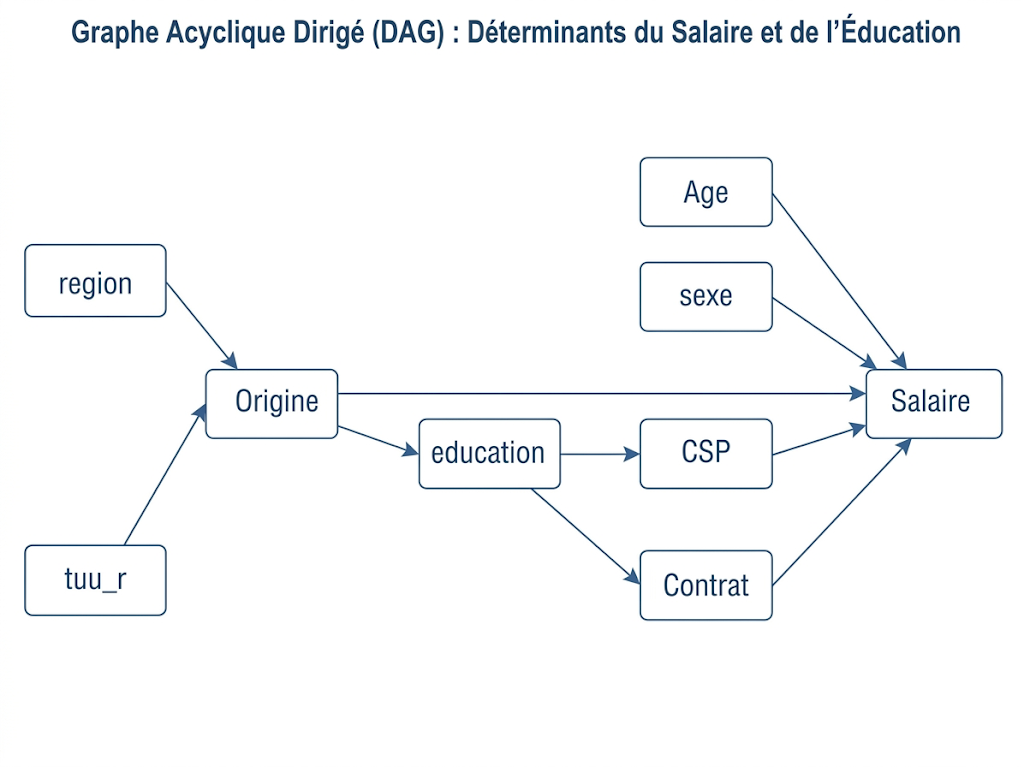
\includegraphics[keepaspectratio]{images/clipboard-2917733682.png}}

\paragraph{\texorpdfstring{\textbf{b)
Interprétation}}{b) Interprétation}}\label{b-interpruxe9tation}

Tous les modèles estimés ne peuvent s'interpréter qu'en termes de
prédiction et non de causalité. En effet, l'hypothèse d'abscence de
biais de sélection est très peu crédible; bien qu'on ait contrôlé par
certaines variables pertinentes.

Les interprétations suivantes, se feront (pour des besoins de
simplicité) uniquement sur les personnes originaires d'afrique.

On va entraîner les deux modèles, mais de façon progressive en ajoutant
des nouvelles variables au fur et à mesure, et voir comment les
coefficients évoluent.

\begin{Shaded}
\begin{Highlighting}[]
\CommentTok{\#{-}{-}{-}{-}{-}{-}{-}{-}{-}{-}{-}{-}{-}{-}{-}{-}{-}{-}{-}{-}QUESTION 1{-}{-}{-}{-}{-}{-}{-}{-}{-}{-}{-}{-}{-}{-}{-}{-}{-}{-}{-}{-}{-}{-}{-}{-}{-}{-}{-}{-}{-}{-}{-}{-}}
\NormalTok{df1 }\OtherTok{\textless{}{-}}\NormalTok{ df }\SpecialCharTok{\%\textgreater{}\%}
  \FunctionTok{filter}\NormalTok{(t }\SpecialCharTok{==} \DecValTok{6}\NormalTok{, acteu }\SpecialCharTok{==} \DecValTok{1}\NormalTok{)}\SpecialCharTok{\%\textgreater{}\%}
  \FunctionTok{mutate}\NormalTok{(}
    \AttributeTok{age2  =}\NormalTok{ age}\SpecialCharTok{\^{}}\DecValTok{2}
\NormalTok{  ) }\SpecialCharTok{\%\textgreater{}\%}
  \FunctionTok{droplevels}\NormalTok{()}


\NormalTok{regression }\OtherTok{\textless{}{-}} \ControlFlowTok{function}\NormalTok{(y, }\AttributeTok{data =}\NormalTok{ df1)\{}
  
  \CommentTok{\# On convertit l\textquotesingle{}argument en caractère }
\NormalTok{  y }\OtherTok{\textless{}{-}} \FunctionTok{deparse}\NormalTok{(}\FunctionTok{substitute}\NormalTok{(y))}
  
  \CommentTok{\# Définition des listes de variables explicatives}
\NormalTok{  rhs1 }\OtherTok{\textless{}{-}} \StringTok{"origine"}
\NormalTok{  rhs2 }\OtherTok{\textless{}{-}} \FunctionTok{c}\NormalTok{(rhs1, }\StringTok{"age"}\NormalTok{, }\StringTok{"age2"}\NormalTok{, }\StringTok{"homme"}\NormalTok{)}
\NormalTok{  rhs3 }\OtherTok{\textless{}{-}} \FunctionTok{c}\NormalTok{(rhs2, }\StringTok{"region"}\NormalTok{, }\StringTok{"tuu\_r"}\NormalTok{)}
\NormalTok{  rhs4 }\OtherTok{\textless{}{-}} \FunctionTok{c}\NormalTok{(rhs3, }\StringTok{"education"}\NormalTok{)}
\NormalTok{  rhs5 }\OtherTok{\textless{}{-}} \FunctionTok{c}\NormalTok{(rhs4, }\StringTok{"csp\_actif"}\NormalTok{, }\StringTok{"contrat"}\NormalTok{)}
  
  \CommentTok{\# Estimation des modèles}
\NormalTok{  m1 }\OtherTok{\textless{}{-}} \FunctionTok{lm\_robust}\NormalTok{(}\FunctionTok{reformulate}\NormalTok{(rhs1, y), }\AttributeTok{data =}\NormalTok{ data)}
\NormalTok{  m2 }\OtherTok{\textless{}{-}} \FunctionTok{lm\_robust}\NormalTok{(}\FunctionTok{reformulate}\NormalTok{(rhs2, y), }\AttributeTok{data =}\NormalTok{ data)}
\NormalTok{  m3 }\OtherTok{\textless{}{-}} \FunctionTok{lm\_robust}\NormalTok{(}\FunctionTok{reformulate}\NormalTok{(rhs3, y), }\AttributeTok{data =}\NormalTok{ data)}
\NormalTok{  m4 }\OtherTok{\textless{}{-}} \FunctionTok{lm\_robust}\NormalTok{(}\FunctionTok{reformulate}\NormalTok{(rhs4, y), }\AttributeTok{data =}\NormalTok{ data)}
\NormalTok{  m5 }\OtherTok{\textless{}{-}} \FunctionTok{lm\_robust}\NormalTok{(}\FunctionTok{reformulate}\NormalTok{(rhs5, y), }\AttributeTok{data =}\NormalTok{ data)}
  
  \CommentTok{\# On regroupe pour le tableau}
\NormalTok{  models }\OtherTok{\textless{}{-}} \FunctionTok{list}\NormalTok{(}
    \StringTok{"modèle(1)"} \OtherTok{=}\NormalTok{ m1, }
    \StringTok{"modèle(2)"} \OtherTok{=}\NormalTok{ m2, }
    \StringTok{"modèle(3)"} \OtherTok{=}\NormalTok{ m3, }
    \StringTok{"modèle(4)"} \OtherTok{=}\NormalTok{ m4, }
    \StringTok{"modèle(5)"} \OtherTok{=}\NormalTok{ m5}
\NormalTok{  )}
  
  \CommentTok{\# Rendu du tableau}
  \FunctionTok{modelsummary}\NormalTok{(}
\NormalTok{    models,}
    \AttributeTok{stars =} \ConstantTok{TRUE}\NormalTok{,}
    \AttributeTok{coef\_omit =} \StringTok{"Intercept"}\NormalTok{,}
    \AttributeTok{gof\_omit =} \StringTok{"AIC|BIC|Log.Lik|F|Std.Errors"}\NormalTok{,}
    \AttributeTok{title =} \FunctionTok{paste}\NormalTok{(}\StringTok{"Analyse de la variable :"}\NormalTok{, y),}
    \AttributeTok{notes =} \StringTok{"Écarts{-}types robustes (HC2)."}
\NormalTok{  )}
  
\NormalTok{\}}
  \CommentTok{\# a) Modèle LOG }
\FunctionTok{regression}\NormalTok{(logsalhoraire)}
\end{Highlighting}
\end{Shaded}

\begin{table}
\centering
\begin{talltblr}[         %% tabularray outer open
caption={Analyse de la variable : logsalhoraire},
note{}={+ p \num{< 0.1}, * p \num{< 0.05}, ** p \num{< 0.01}, *** p \num{< 0.001}},
note{ }={Écarts-types robustes (HC2).},
]                     %% tabularray outer close
{                     %% tabularray inner open
colspec={Q[]Q[]Q[]Q[]Q[]Q[]},
hline{2}={1-6}{solid, black, 0.05em},
hline{66}={1-6}{solid, black, 0.05em},
hline{1}={1-6}{solid, black, 0.08em},
hline{70}={1-6}{solid, black, 0.08em},
column{2-6}={}{halign=c},
column{1}={}{halign=l},
}                     %% tabularray inner close
& modèle(1) & modèle(2) & modèle(3) & modèle(4) & modèle(5) \\
origine03 & \num{0.120}* & \num{0.123}* & \num{0.121}* & \num{0.078}+ & \num{0.105}* \\
& (\num{0.052}) & (\num{0.050}) & (\num{0.050}) & (\num{0.044}) & (\num{0.043}) \\
origine04 & \num{-0.004} & \num{-0.007} & \num{-0.028} & \num{0.036} & \num{0.051}* \\
& (\num{0.026}) & (\num{0.025}) & (\num{0.026}) & (\num{0.024}) & (\num{0.023}) \\
origine05 & \num{-0.023} & \num{-0.038} & \num{-0.054} & \num{-0.097}+ & \num{-0.026} \\
& (\num{0.056}) & (\num{0.052}) & (\num{0.052}) & (\num{0.053}) & (\num{0.045}) \\
origine06 & \num{-0.041} & \num{-0.050}+ & \num{-0.104}** & \num{-0.039} & \num{-0.009} \\
& (\num{0.031}) & (\num{0.030}) & (\num{0.032}) & (\num{0.029}) & (\num{0.024}) \\
origine07 & \num{-0.178}*** & \num{-0.153}*** & \num{-0.222}*** & \num{-0.155}** & \num{-0.067}+ \\
& (\num{0.048}) & (\num{0.046}) & (\num{0.045}) & (\num{0.048}) & (\num{0.041}) \\
origine08 & \num{0.095} & \num{0.104} & \num{0.051} & \num{0.081} & \num{0.090} \\
& (\num{0.083}) & (\num{0.078}) & (\num{0.076}) & (\num{0.062}) & (\num{0.062}) \\
origine09 & \num{-0.184}* & \num{-0.155}* & \num{-0.169}* & \num{-0.054} & \num{-0.040} \\
& (\num{0.079}) & (\num{0.071}) & (\num{0.078}) & (\num{0.064}) & (\num{0.057}) \\
origine10 & \num{-0.010} & \num{-0.001} & \num{-0.028} & \num{-0.083} & \num{-0.045} \\
& (\num{0.099}) & (\num{0.096}) & (\num{0.101}) & (\num{0.080}) & (\num{0.075}) \\
origine99 & \num{-0.140}** & \num{-0.134}** & \num{-0.154}*** & \num{-0.070}+ & \num{-0.046} \\
& (\num{0.046}) & (\num{0.044}) & (\num{0.043}) & (\num{0.039}) & (\num{0.036}) \\
age &  & \num{0.028}*** & \num{0.029}*** & \num{0.027}*** & \num{0.016}** \\
&  & (\num{0.006}) & (\num{0.006}) & (\num{0.006}) & (\num{0.006}) \\
age2 &  & \num{-0.000}*** & \num{-0.000}*** & \num{-0.000}** & \num{-0.000}+ \\
&  & (\num{0.000}) & (\num{0.000}) & (\num{0.000}) & (\num{0.000}) \\
homme &  & \num{0.134}*** & \num{0.136}*** & \num{0.164}*** & \num{0.101}*** \\
&  & (\num{0.012}) & (\num{0.012}) & (\num{0.011}) & (\num{0.011}) \\
region &  &  & \num{-0.004}+ & \num{-0.000} & \num{-0.001} \\
&  &  & (\num{0.002}) & (\num{0.002}) & (\num{0.002}) \\
tuu\_r2 &  &  & \num{-0.033}+ & \num{-0.030}+ & \num{-0.028}+ \\
&  &  & (\num{0.017}) & (\num{0.016}) & (\num{0.015}) \\
tuu\_r3 &  &  & \num{0.015} & \num{-0.002} & \num{0.002} \\
&  &  & (\num{0.018}) & (\num{0.016}) & (\num{0.015}) \\
tuu\_r4 &  &  & \num{0.059}*** & \num{0.004} & \num{-0.010} \\
&  &  & (\num{0.017}) & (\num{0.016}) & (\num{0.015}) \\
tuu\_r5 &  &  & \num{0.150}*** & \num{0.095}*** & \num{0.046}* \\
&  &  & (\num{0.025}) & (\num{0.022}) & (\num{0.021}) \\
education3 &  &  &  & \num{-0.135}*** & \num{-0.032}+ \\
&  &  &  & (\num{0.019}) & (\num{0.018}) \\
education4 &  &  &  & \num{-0.264}*** & \num{-0.087}*** \\
&  &  &  & (\num{0.019}) & (\num{0.019}) \\
education5 &  &  &  & \num{-0.391}*** & \num{-0.147}*** \\
&  &  &  & (\num{0.017}) & (\num{0.020}) \\
education6 &  &  &  & \num{-0.406}*** & \num{-0.157}*** \\
&  &  &  & (\num{0.027}) & (\num{0.027}) \\
education7 &  &  &  & \num{-0.515}*** & \num{-0.240}*** \\
&  &  &  & (\num{0.022}) & (\num{0.025}) \\
csp\_actif3 &  &  &  &  & \num{0.928} \\
&  &  &  &  & (\num{0.820}) \\
csp\_actif4 &  &  &  &  & \num{0.710} \\
&  &  &  &  & (\num{0.820}) \\
csp\_actif5 &  &  &  &  & \num{0.501} \\
&  &  &  &  & (\num{0.820}) \\
csp\_actif6 &  &  &  &  & \num{0.558} \\
&  &  &  &  & (\num{0.820}) \\
contrat0 &  &  &  &  & \num{-0.019} \\
&  &  &  &  & (\num{0.124}) \\
contrat1 &  &  &  &  & \num{-0.083} \\
&  &  &  &  & (\num{0.124}) \\
contrat2 &  &  &  &  & \num{-0.249}+ \\
&  &  &  &  & (\num{0.127}) \\
contrat3 &  &  &  &  & \num{-0.261}+ \\
&  &  &  &  & (\num{0.148}) \\
contrat4 &  &  &  &  & \num{-0.118} \\
&  &  &  &  & (\num{0.133}) \\
contrat5 &  &  &  &  & \num{-0.482}** \\
&  &  &  &  & (\num{0.184}) \\
Num.Obs. & \num{4046} & \num{4046} & \num{4046} & \num{4046} & \num{4046} \\
R2 & \num{0.008} & \num{0.062} & \num{0.083} & \num{0.251} & \num{0.361} \\
R2 Adj. & \num{0.006} & \num{0.059} & \num{0.079} & \num{0.247} & \num{0.356} \\
RMSE & \num{0.40} & \num{0.39} & \num{0.38} & \num{0.35} & \num{0.32} \\
\end{talltblr}
\end{table}

\begin{Shaded}
\begin{Highlighting}[]
\CommentTok{\# a) Modèle en niveau }
\FunctionTok{regression}\NormalTok{(salhoraire)}
\end{Highlighting}
\end{Shaded}

\begin{table}
\centering
\begin{talltblr}[         %% tabularray outer open
caption={Analyse de la variable : salhoraire},
note{}={+ p \num{< 0.1}, * p \num{< 0.05}, ** p \num{< 0.01}, *** p \num{< 0.001}},
note{ }={Écarts-types robustes (HC2).},
]                     %% tabularray outer close
{                     %% tabularray inner open
colspec={Q[]Q[]Q[]Q[]Q[]Q[]},
hline{2}={1-6}{solid, black, 0.05em},
hline{66}={1-6}{solid, black, 0.05em},
hline{1}={1-6}{solid, black, 0.08em},
hline{70}={1-6}{solid, black, 0.08em},
column{2-6}={}{halign=c},
column{1}={}{halign=l},
}                     %% tabularray inner close
& modèle(1) & modèle(2) & modèle(3) & modèle(4) & modèle(5) \\
origine03 & \num{1.464}+ & \num{1.460}* & \num{1.429}+ & \num{0.798} & \num{1.083} \\
& (\num{0.757}) & (\num{0.742}) & (\num{0.730}) & (\num{0.659}) & (\num{0.674}) \\
origine04 & \num{0.055} & \num{0.056} & \num{-0.237} & \num{0.546} & \num{0.724} \\
& (\num{0.583}) & (\num{0.589}) & (\num{0.605}) & (\num{0.585}) & (\num{0.578}) \\
origine05 & \num{-0.304} & \num{-0.562} & \num{-0.777} & \num{-1.313}* & \num{-0.424} \\
& (\num{0.730}) & (\num{0.654}) & (\num{0.642}) & (\num{0.664}) & (\num{0.574}) \\
origine06 & \num{-0.752}+ & \num{-0.835}* & \num{-1.564}*** & \num{-0.804}* & \num{-0.451} \\
& (\num{0.398}) & (\num{0.398}) & (\num{0.431}) & (\num{0.397}) & (\num{0.333}) \\
origine07 & \num{-1.940}** & \num{-1.645}* & \num{-2.558}*** & \num{-1.782}** & \num{-0.797} \\
& (\num{0.688}) & (\num{0.662}) & (\num{0.647}) & (\num{0.667}) & (\num{0.564}) \\
origine08 & \num{1.607} & \num{1.887} & \num{1.179} & \num{1.429} & \num{1.469} \\
& (\num{1.428}) & (\num{1.378}) & (\num{1.340}) & (\num{1.154}) & (\num{1.135}) \\
origine09 & \num{-2.303}** & \num{-1.974}** & \num{-2.223}** & \num{-0.900} & \num{-0.722} \\
& (\num{0.807}) & (\num{0.734}) & (\num{0.838}) & (\num{0.631}) & (\num{0.590}) \\
origine10 & \num{0.342} & \num{0.560} & \num{0.206} & \num{-0.624} & \num{-0.227} \\
& (\num{1.329}) & (\num{1.305}) & (\num{1.367}) & (\num{1.124}) & (\num{1.028}) \\
origine99 & \num{-1.579}** & \num{-1.576}** & \num{-1.822}*** & \num{-0.787}+ & \num{-0.539} \\
& (\num{0.521}) & (\num{0.496}) & (\num{0.477}) & (\num{0.419}) & (\num{0.375}) \\
age &  & \num{0.068} & \num{0.084} & \num{0.073} & \num{-0.046} \\
&  & (\num{0.149}) & (\num{0.151}) & (\num{0.148}) & (\num{0.154}) \\
age2 &  & \num{0.000} & \num{0.000} & \num{0.001} & \num{0.001} \\
&  & (\num{0.002}) & (\num{0.002}) & (\num{0.002}) & (\num{0.002}) \\
homme &  & \num{1.592}*** & \num{1.608}*** & \num{1.964}*** & \num{1.260}*** \\
&  & (\num{0.173}) & (\num{0.172}) & (\num{0.163}) & (\num{0.161}) \\
region &  &  & \num{-0.061}* & \num{-0.020} & \num{-0.026} \\
&  &  & (\num{0.028}) & (\num{0.026}) & (\num{0.025}) \\
tuu\_r2 &  &  & \num{-0.330} & \num{-0.295} & \num{-0.280} \\
&  &  & (\num{0.249}) & (\num{0.236}) & (\num{0.228}) \\
tuu\_r3 &  &  & \num{0.084} & \num{-0.141} & \num{-0.085} \\
&  &  & (\num{0.237}) & (\num{0.219}) & (\num{0.207}) \\
tuu\_r4 &  &  & \num{0.877}*** & \num{0.131} & \num{-0.082} \\
&  &  & (\num{0.254}) & (\num{0.236}) & (\num{0.227}) \\
tuu\_r5 &  &  & \num{1.993}*** & \num{1.232}*** & \num{0.602}+ \\
&  &  & (\num{0.386}) & (\num{0.352}) & (\num{0.338}) \\
education3 &  &  &  & \num{-2.210}*** & \num{-0.803}** \\
&  &  &  & (\num{0.311}) & (\num{0.293}) \\
education4 &  &  &  & \num{-3.794}*** & \num{-1.543}*** \\
&  &  &  & (\num{0.284}) & (\num{0.285}) \\
education5 &  &  &  & \num{-5.376}*** & \num{-2.318}*** \\
&  &  &  & (\num{0.259}) & (\num{0.280}) \\
education6 &  &  &  & \num{-5.588}*** & \num{-2.524}*** \\
&  &  &  & (\num{0.387}) & (\num{0.391}) \\
education7 &  &  &  & \num{-6.367}*** & \num{-2.948}*** \\
&  &  &  & (\num{0.332}) & (\num{0.352}) \\
csp\_actif3 &  &  &  &  & \num{7.601} \\
&  &  &  &  & (\num{5.814}) \\
csp\_actif4 &  &  &  &  & \num{4.236} \\
&  &  &  &  & (\num{5.809}) \\
csp\_actif5 &  &  &  &  & \num{2.138} \\
&  &  &  &  & (\num{5.808}) \\
csp\_actif6 &  &  &  &  & \num{2.545} \\
&  &  &  &  & (\num{5.812}) \\
contrat0 &  &  &  &  & \num{-1.935} \\
&  &  &  &  & (\num{2.982}) \\
contrat1 &  &  &  &  & \num{-2.496} \\
&  &  &  &  & (\num{2.994}) \\
contrat2 &  &  &  &  & \num{-4.138} \\
&  &  &  &  & (\num{3.043}) \\
contrat3 &  &  &  &  & \num{-4.107} \\
&  &  &  &  & (\num{3.104}) \\
contrat4 &  &  &  &  & \num{-2.700} \\
&  &  &  &  & (\num{3.046}) \\
contrat5 &  &  &  &  & \num{-6.230}+ \\
&  &  &  &  & (\num{3.385}) \\
Num.Obs. & \num{4046} & \num{4046} & \num{4046} & \num{4046} & \num{4046} \\
R2 & \num{0.006} & \num{0.046} & \num{0.065} & \num{0.200} & \num{0.279} \\
R2 Adj. & \num{0.004} & \num{0.043} & \num{0.061} & \num{0.196} & \num{0.273} \\
RMSE & \num{5.71} & \num{5.59} & \num{5.54} & \num{5.12} & \num{4.86} \\
\end{talltblr}
\end{table}

Toutes choses égales par ailleurs, le modèle 1 prédit qu'un individu
originaire d'Afrique gagne en moyenne \textbf{8,40 \$/h de moins} qu'un
Français (soit une pénalité de \textbf{17,8 \%} selon la spécification
en log). Ce résultat est statistiquement significatif au seuil de
\textbf{1 \%}. L'ajout des variables de contrôle (âge, sexe et zone
géographique) affine l'estimation, mais le signe, l'ampleur et la
significativité de l'effet demeurent \textbf{robustes}.

En contrôlant en plus par l'\textbf{éducation} (modèle 4), l'écart se
réduit légèrement mais reste massif : un individu originaire d'Afrique
gagne désormais, toutes choses égales par ailleurs, \textbf{7,71 \$/h de
moins} qu'un Français (soit \textbf{15 \%} en moins dans le modèle en
log). La persistance de cet effet, même à diplôme identique, suggère
qu'une part prépondérante de l'inégalité salariale est directe et ne
s'explique pas uniquement par des différences de capital humain. L'ajout
de \textbf{éducation} provoque en plus une hausse substantielle du
\(R^2\) (passant de \textbf{8,3\%} à \textbf{25,1\%}). Cette progression
démontre que le capital humain est le principal facteur explicatif de la
variance des salaires dans notre échantillon.

Enfin, le modèle 5 intègre la CSP et le type de contrat. L'effet de
l'origine devient beaucoup plus fragile. Le coefficient n'est plus
significatif dans le modèle en niveau et ne l'est qu'au seuil de
\textbf{10 \%} dans le modèle en log. Ce résultat suggère qu'à CSP et
type de contrat identiques, l'écart de salaire horaire tend à s'estomper
statistiquement. En d'autres termes, l'essentiel du désavantage lié à
l'origine constaté dans les modèles précédents semble transiter par une
\textbf{ségrégation professionnelle} (accès plus difficile aux postes
qualifiés et aux contrats stables) plutôt que par une inégalité de
rémunération directe au sein d'un même poste.

\paragraph{\texorpdfstring{\textbf{c) Canaux de transmission de l'effet
de l'origine sur le
salaire}}{c) Canaux de transmission de l'effet de l'origine sur le salaire}}\label{c-canaux-de-transmission-de-leffet-de-lorigine-sur-le-salaire}

Les régressions précédentes met en évidence une pénalité de 17,8\% pour
les individus d'origine africaine par rapport aux français (modèle 1).
L'introduction du niveau d'éducation (modèle 4), ne réduit cet écart
qu'à 15,5\%; ce qui suggère que la disparité salariale ne résulte pas
principalement d'une différence de capital humain. L'éducation, bien que
élément important du salaire, n'explique qu'une faible part de
l'inégalité liée à l'origine.

En ajoutant la CSP et le type de contrat (modèle 5), on observe un
effondrement de l'amplitude des coefficients de l'éducation, et une
chute de la pénalité à 6,7\%. Cela prouve qu'une grande partie du
rendement de l'éducation transite par le canal de \textbf{l'insertion
professionnelle}. La CSP et le contrat absorbent donc une partie de
l'effet de l'éducation (et de l'origine).

Finalement, ces résultats révèlent 02 possibles formes de
discrimination. D'une part, \textbf{une discrimination à l'embauche
(prépondérante):} l'origine impacterait l'obtention de statuts
particuliers (cadres) ou de contrats stables (CDI). D'autre part,
\textbf{une discrimination à la rémunération (pure)}, qui subsiste même
à poste et contrat identiques.

\subsubsection{Question 2 -- Inclure le niveau de diplôme comme variable
de
contrôle}\label{question-2-inclure-le-niveau-de-dipluxf4me-comme-variable-de-contruxf4le}

\paragraph{\texorpdfstring{\textbf{a) Problème qui peut survenir en
contrôlant par le niveau de
diplôme}}{a) Problème qui peut survenir en contrôlant par le niveau de diplôme}}\label{a-probluxe8me-qui-peut-survenir-en-contruxf4lant-par-le-niveau-de-dipluxf4me}

Dans cette partie, on s'intéresse à l'effet de l'origine sur le salaire.
Si la réalité est telle que l'origine influence le salaire à travers le
niveau d'éducation, alors en contrôlant par l'éducation, on commet un
\textbf{biais de variable incluse} puisqu'on bloque un chemin causal.
Par conséquent, le coefficient de Origine est biaisé vers le bas, et ne
mesure que l'effet ``\textbf{à niveau d'éducation égal}''.

De plus, l'éducation est certainement endogène ici, car il n'est
certainement pas choisi au hasard par les individus (actifs occupés) de
notre échantillon. Il est donc correlé aux facteurs inobservés.

\paragraph{\texorpdfstring{\textbf{b) Variables disponibles pour
instrumenter
l'éducation}}{b) Variables disponibles pour instrumenter l'éducation}}\label{b-variables-disponibles-pour-instrumenter-luxe9ducation}

Comme instruments, on peut utiliser: la catégorie socio-professionnelle
des parents.

\begin{itemize}
\item
  Pertinence: La CSP des parents devrait être correlée au niveau
  d'éducation de l'enfant, notamment en raison de l'héritage culturel
  et/ou la reproduction sociale. Un enfant ayant des parents qui sont
  professeurs d'université par exemple, aura tendance à poursuivre ses
  études jusqu'au master au moins (ou Doctorat), contrairement à un
  enfant d'ouvriers.
\item
  Exogénéité: Elle repose sur une hypothèse qui est discutable: l\emph{a
  profession des parents n'influence le salaire de l'enfant que par le
  niveau diplôme}. En pratique, les enfants peuvent très biens
  bénéficier des ``connexions'' ou du ``réseau'' de leurs parents pour
  décrocher des emplois bien rémunérés.

\begin{Shaded}
\begin{Highlighting}[]
\CommentTok{\#{-}{-}{-}{-}{-}{-}{-}{-}{-}{-}{-}{-}{-}{-}{-}{-}{-}{-}{-}{-}QUESTION 2{-}{-}{-}{-}{-}{-}{-}{-}{-}{-}{-}{-}{-}{-}{-}{-}{-}{-}{-}{-}{-}{-}{-}{-}{-}{-}{-}{-}{-}}

          \CommentTok{\#{-}{-}{-}{-}{-}{-}{-}{-}Pertinence{-}{-}{-}{-}{-}{-}{-}{-}{-}{-}}
\NormalTok{m\_iv }\OtherTok{\textless{}{-}} \FunctionTok{iv\_robust}\NormalTok{(}
\NormalTok{  logsalhoraire }\SpecialCharTok{\textasciitilde{}}\NormalTok{ origine }\SpecialCharTok{+}\NormalTok{ age }\SpecialCharTok{+}\NormalTok{ age2 }\SpecialCharTok{+}\NormalTok{ homme }\SpecialCharTok{+}\NormalTok{ region }\SpecialCharTok{+}\NormalTok{ tuu\_r }\SpecialCharTok{+}\NormalTok{ education }\SpecialCharTok{|} 
\NormalTok{    origine }\SpecialCharTok{+}\NormalTok{ age }\SpecialCharTok{+}\NormalTok{ age2 }\SpecialCharTok{+}\NormalTok{ homme }\SpecialCharTok{+}\NormalTok{ region }\SpecialCharTok{+}\NormalTok{ tuu\_r }\SpecialCharTok{+}\NormalTok{ csp\_mere,}
  \AttributeTok{data =}\NormalTok{ df1,}
  \AttributeTok{diagnostics =} \ConstantTok{TRUE} \CommentTok{\# TRÈS IMPORTANT pour avoir le F{-}test}
\NormalTok{)}

\FunctionTok{summary}\NormalTok{(m\_iv)}
\end{Highlighting}
\end{Shaded}

\begin{verbatim}

Call:
iv_robust(formula = logsalhoraire ~ origine + age + age2 + homme + 
    region + tuu_r + education | origine + age + age2 + homme + 
    region + tuu_r + csp_mere, data = df1, diagnostics = TRUE)

Standard error type:  HC2 

Coefficients:
              Estimate Std. Error t value  Pr(>|t|)   CI Lower   CI Upper   DF
(Intercept)  3.1947186  1.745e-01 18.3111 5.269e-72  2.8526634  3.537e+00 4023
origine03    0.0769272  4.860e-02  1.5828 1.135e-01 -0.0183603  1.722e-01 4023
origine04    0.0532342  3.351e-02  1.5887 1.122e-01 -0.0124590  1.189e-01 4023
origine05   -0.0971312  5.949e-02 -1.6326 1.026e-01 -0.2137734  1.951e-02 4023
origine06   -0.0053161  3.659e-02 -0.1453 8.845e-01 -0.0770596  6.643e-02 4023
origine07   -0.1435007  6.209e-02 -2.3111 2.088e-02 -0.2652342 -2.177e-02 4023
origine08    0.1033593  7.841e-02  1.3182 1.875e-01 -0.0503720  2.571e-01 4023
origine09   -0.0174043  9.731e-02 -0.1789 8.581e-01 -0.2081770  1.734e-01 4023
origine10   -0.0848880  8.911e-02 -0.9526 3.408e-01 -0.2595944  8.982e-02 4023
origine99   -0.0713317  5.421e-02 -1.3159 1.883e-01 -0.1776061  3.494e-02 4023
age          0.0296382  7.852e-03  3.7747 1.625e-04  0.0142442  4.503e-02 4023
age2        -0.0002161  8.987e-05 -2.4049 1.622e-02 -0.0003923 -3.993e-05 4023
homme        0.1781293  1.583e-02 11.2528 6.050e-29  0.1470940  2.092e-01 4023
region       0.0007926  2.287e-03  0.3465 7.290e-01 -0.0036920  5.277e-03 4023
tuu_r2      -0.0359253  1.823e-02 -1.9702 4.888e-02 -0.0716745 -1.762e-04 4023
tuu_r3      -0.0057549  1.837e-02 -0.3133 7.541e-01 -0.0417671  3.026e-02 4023
tuu_r4      -0.0117801  1.847e-02 -0.6377 5.237e-01 -0.0479948  2.443e-02 4023
tuu_r5       0.0814329  2.835e-02  2.8725 4.094e-03  0.0258531  1.370e-01 4023
education3  -0.1766843  1.724e-01 -1.0248 3.055e-01 -0.5146937  1.613e-01 4023
education4  -0.1980281  1.677e-01 -1.1809 2.377e-01 -0.5267982  1.307e-01 4023
education5  -0.5245113  1.143e-01 -4.5894 4.580e-06 -0.7485774 -3.004e-01 4023
education6  -0.1725488  2.899e-01 -0.5953 5.517e-01 -0.7408197  3.957e-01 4023
education7  -0.7114559  1.375e-01 -5.1727 2.420e-07 -0.9811112 -4.418e-01 4023

Multiple R-squared:  0.1797 ,   Adjusted R-squared:  0.1752 
F-statistic: 24.02 on 22 and 4023 DF,  p-value: < 2.2e-16

Diagnostics:
                              numdf dendf  value p.value    
Weak instruments (education3)    31  3997 10.555  <2e-16 ***
Weak instruments (education4)    31  3997  9.941  <2e-16 ***
Weak instruments (education5)    31  3997 12.457  <2e-16 ***
Weak instruments (education6)    31  3997  5.550  <2e-16 ***
Weak instruments (education7)    31  3997  9.497  <2e-16 ***
Wu-Hausman                        5  4018  1.790  0.1114    
Overidentifying                  26    NA 35.747  0.0964 .  
---
Signif. codes:  0 '***' 0.001 '**' 0.01 '*' 0.05 '.' 0.1 ' ' 1
\end{verbatim}
\end{itemize}

Les tests de diagnostic indiquent que nos instruments (CSP de la mère)
sont globalement \textbf{pertinents}. Pour la plupart des niveaux
d'éducation, la statistique F est proche ou supérieure à \textbf{10}, ce
qui correspond à la règle empirique usuelle pour écarter le risque
d'instruments faibles. On note toutefois une faiblesse relative pour le
niveau \texttt{education6} (\(F = 5,55\)). Néanmoins, les p-valeurs
extrêmement faibles (\(< 2e-16\)) sur l'ensemble des modalités
confirment que la CSP des parents reste un prédicteur significatif du
parcours scolaire, permettant ainsi une identification du modèle.

De plus, le test de sargan confirme (au seuil de 10\%), que la CSP des
parents n'impacte le salaire qu'à travers le niveau d'education de
l'enfant. Le test de Wu-Hausmann suggère que l'estimateur MCO n'était
pas nécessairement biaisé de mainère significative par des variables
omises. Dans ce cas, l'approche IV sert principalement de \textbf{test
de robustesse.}

\paragraph{\texorpdfstring{\textbf{b) Interprétation des
résultats}}{b) Interprétation des résultats}}\label{b-interpruxe9tation-des-ruxe9sultats}

\begin{Shaded}
\begin{Highlighting}[]
        \CommentTok{\#{-}{-}{-}{-}{-}{-}{-}Estimation{-}{-}{-}{-}{-}{-}{-}{-}{-}{-}{-}{-}}
\NormalTok{m\_ols }\OtherTok{\textless{}{-}} \FunctionTok{lm}\NormalTok{(logsalhoraire }\SpecialCharTok{\textasciitilde{}}\NormalTok{ origine }\SpecialCharTok{+}\NormalTok{ age }\SpecialCharTok{+}\NormalTok{ age2 }\SpecialCharTok{+}\NormalTok{ homme }\SpecialCharTok{+}\NormalTok{ region }\SpecialCharTok{+}\NormalTok{ tuu\_r }\SpecialCharTok{+}\NormalTok{ education, }\AttributeTok{data =}\NormalTok{ df1)}
\NormalTok{models\_iv }\OtherTok{\textless{}{-}} \FunctionTok{list}\NormalTok{(}
  \StringTok{"Modèle 4"} \OtherTok{=}\NormalTok{ m\_ols, }\CommentTok{\# le modèle précédent}
  \StringTok{"IV (2SLS)"} \OtherTok{=}\NormalTok{ m\_iv}
\NormalTok{)}

\FunctionTok{modelsummary}\NormalTok{(}
\NormalTok{  models\_iv,}
  \AttributeTok{stars =} \ConstantTok{TRUE}\NormalTok{,}
  \AttributeTok{coef\_omit =} \StringTok{"Intercept"}\NormalTok{,}
  \AttributeTok{gof\_omit =} \StringTok{"AIC|BIC|Log.Lik|F|Std.Errors"}\NormalTok{,}
  \AttributeTok{title =} \StringTok{"Comparaison MCO vs Variables Instrumentales"}\NormalTok{,}
  \AttributeTok{notes =} \StringTok{"Instruments : CSP de la mere."}
\NormalTok{)}
\end{Highlighting}
\end{Shaded}

\begin{table}
\centering
\begin{talltblr}[         %% tabularray outer open
caption={Comparaison MCO vs Variables Instrumentales},
note{}={+ p \num{< 0.1}, * p \num{< 0.05}, ** p \num{< 0.01}, *** p \num{< 0.001}},
note{ }={Instruments : CSP de la mere.},
]                     %% tabularray outer close
{                     %% tabularray inner open
colspec={Q[]Q[]Q[]},
hline{2}={1-3}{solid, black, 0.05em},
hline{46}={1-3}{solid, black, 0.05em},
hline{1}={1-3}{solid, black, 0.08em},
hline{50}={1-3}{solid, black, 0.08em},
column{2-3}={}{halign=c},
column{1}={}{halign=l},
}                     %% tabularray inner close
& Modèle 4 & IV (2SLS) \\
origine03 & \num{0.078}+ & \num{0.077} \\
& (\num{0.046}) & (\num{0.049}) \\
origine04 & \num{0.036} & \num{0.053} \\
& (\num{0.024}) & (\num{0.034}) \\
origine05 & \num{-0.097}+ & \num{-0.097} \\
& (\num{0.049}) & (\num{0.059}) \\
origine06 & \num{-0.039} & \num{-0.005} \\
& (\num{0.032}) & (\num{0.037}) \\
origine07 & \num{-0.155}*** & \num{-0.144}* \\
& (\num{0.046}) & (\num{0.062}) \\
origine08 & \num{0.081} & \num{0.103} \\
& (\num{0.064}) & (\num{0.078}) \\
origine09 & \num{-0.054} & \num{-0.017} \\
& (\num{0.085}) & (\num{0.097}) \\
origine10 & \num{-0.083} & \num{-0.085} \\
& (\num{0.070}) & (\num{0.089}) \\
origine99 & \num{-0.070}+ & \num{-0.071} \\
& (\num{0.040}) & (\num{0.054}) \\
age & \num{0.027}*** & \num{0.030}*** \\
& (\num{0.004}) & (\num{0.008}) \\
age2 & \num{-0.000}*** & \num{-0.000}* \\
& (\num{0.000}) & (\num{0.000}) \\
homme & \num{0.164}*** & \num{0.178}*** \\
& (\num{0.011}) & (\num{0.016}) \\
region & \num{-0.000} & \num{0.001} \\
& (\num{0.002}) & (\num{0.002}) \\
tuu\_r2 & \num{-0.030}+ & \num{-0.036}* \\
& (\num{0.016}) & (\num{0.018}) \\
tuu\_r3 & \num{-0.002} & \num{-0.006} \\
& (\num{0.017}) & (\num{0.018}) \\
tuu\_r4 & \num{0.004} & \num{-0.012} \\
& (\num{0.015}) & (\num{0.018}) \\
tuu\_r5 & \num{0.095}*** & \num{0.081}** \\
& (\num{0.022}) & (\num{0.028}) \\
education3 & \num{-0.135}*** & \num{-0.177} \\
& (\num{0.018}) & (\num{0.172}) \\
education4 & \num{-0.264}*** & \num{-0.198} \\
& (\num{0.018}) & (\num{0.168}) \\
education5 & \num{-0.391}*** & \num{-0.525}*** \\
& (\num{0.017}) & (\num{0.114}) \\
education6 & \num{-0.406}*** & \num{-0.173} \\
& (\num{0.027}) & (\num{0.290}) \\
education7 & \num{-0.515}*** & \num{-0.711}*** \\
& (\num{0.021}) & (\num{0.138}) \\
Num.Obs. & \num{4046} & \num{4046} \\
R2 & \num{0.251} & \num{0.180} \\
R2 Adj. & \num{0.247} & \num{0.175} \\
RMSE & \num{0.35} & \num{0.36} \\
\end{talltblr}
\end{table}

Le passage du MCO à l'IV montre une \textbf{grande stabilité des
coefficients}. D'un point de vue quantitatif, à caractéristiques égales,
un africain a un salaire horaire inférieur de 14,4\% à celui d'un
français.. Ce résultat étant significatif au seuil de 5\%.

Ces résultats confirment que l'origine a un effet direct sur la
rémunération, indépendant du parcours scolaire. Enfin, notons que l'IV
et les MCO produisent des résultats très similaires (voir coef.
Origine), comme le suggérait le test de Wu-Hausman.

\subsubsection{Question 3 -- On reconsidère la structure de
panel}\label{question-3-on-reconsiduxe8re-la-structure-de-panel}

On considère les observations au premier et au dernier trimestre pour
les individus actifs occupés.

\paragraph{\texorpdfstring{\textbf{a) Regression
Pooled}}{a) Regression Pooled}}\label{a-regression-pooled}

Si l'on suppose l'exogénéité des résidus et effets fixes individuels,
alors le modèle approprié est une ``pooled OLS''. Dans ce cadre, le
coefficient \(\beta\) de la régression est convergent et sans biais.

\begin{Shaded}
\begin{Highlighting}[]
 \CommentTok{\#{-}{-}{-}a) Modèle avec exogénéité des résidus et des effets fixes individuels{-}{-}{-}}
\NormalTok{df\_panel }\OtherTok{\textless{}{-}}\NormalTok{ df }\SpecialCharTok{\%\textgreater{}\%}
  \FunctionTok{filter}\NormalTok{(t }\SpecialCharTok{\%in\%} \FunctionTok{c}\NormalTok{(}\DecValTok{1}\NormalTok{, }\DecValTok{6}\NormalTok{), acteu }\SpecialCharTok{==} \DecValTok{1}\NormalTok{) }\SpecialCharTok{\%\textgreater{}\%}
  \FunctionTok{mutate}\NormalTok{(}\AttributeTok{age2 =}\NormalTok{ age}\SpecialCharTok{\^{}}\DecValTok{2}\NormalTok{) }\SpecialCharTok{\%\textgreater{}\%}
  \FunctionTok{group\_by}\NormalTok{(id\_individu) }\SpecialCharTok{\%\textgreater{}\%}
  \FunctionTok{filter}\NormalTok{(}\FunctionTok{n}\NormalTok{() }\SpecialCharTok{==} \DecValTok{2}\NormalTok{) }\SpecialCharTok{\%\textgreater{}\%}
  \FunctionTok{ungroup}\NormalTok{()}

      \CommentTok{\#Estimation MCO Empilé (Pooled OLS)}

\NormalTok{m3a }\OtherTok{\textless{}{-}} \FunctionTok{plm}\NormalTok{(}
\NormalTok{  logsalhoraire }\SpecialCharTok{\textasciitilde{}}\NormalTok{ origine }\SpecialCharTok{+}\NormalTok{ age }\SpecialCharTok{+}\NormalTok{ age2 }\SpecialCharTok{+}\NormalTok{ homme }\SpecialCharTok{+}\NormalTok{ region }\SpecialCharTok{+}\NormalTok{ tuu\_r }\SpecialCharTok{+}\NormalTok{ education,}
  \AttributeTok{data =}\NormalTok{ df\_panel,}
  \AttributeTok{model =} \StringTok{"pooling"}
\NormalTok{)}
\end{Highlighting}
\end{Shaded}

\begin{verbatim}
Warning in pdata.frame(data, index = index, ...): duplicate couples (id-time) in resulting pdata.frame
 to find out which, use, e.g., table(index(your_pdataframe), useNA = "ifany")
\end{verbatim}

\begin{Shaded}
\begin{Highlighting}[]
\CommentTok{\# Ecarts{-}types robustes (Clustered par individu)}
\FunctionTok{summary}\NormalTok{(m3a, }\AttributeTok{vcov =} \FunctionTok{vcovHC}\NormalTok{(m3a, }\AttributeTok{type =} \StringTok{"HC1"}\NormalTok{, }\AttributeTok{cluster =} \StringTok{"group"}\NormalTok{))}
\end{Highlighting}
\end{Shaded}

\begin{verbatim}
Pooling Model

Note: Coefficient variance-covariance matrix supplied: vcovHC(m3a, type = "HC1", cluster = "group")

Call:
plm(formula = logsalhoraire ~ origine + age + age2 + homme + 
    region + tuu_r + education, data = df_panel, model = "pooling")

Unbalanced Panel: n = 2813, T = 1-4, N = 7625

Residuals:
       Min.     1st Qu.      Median     3rd Qu.        Max. 
-1.99522426 -0.17975937  0.00099268  0.18956312  2.74825917 

Coefficients:
               Estimate  Std. Error  t-value  Pr(>|t|)    
(Intercept)  3.0990e+00  9.7308e-02  31.8476 < 2.2e-16 ***
origine03    4.1265e-02  4.5975e-02   0.8975  0.369462    
origine04    3.2061e-02  2.1755e-02   1.4737  0.140597    
origine05   -5.1394e-02  4.5876e-02  -1.1203  0.262624    
origine06   -6.6935e-02  2.9660e-02  -2.2567  0.024052 *  
origine07   -1.5384e-01  4.7924e-02  -3.2100  0.001333 ** 
origine08   -1.1443e-03  4.8971e-02  -0.0234  0.981358    
origine09   -5.4429e-02  5.7776e-02  -0.9421  0.346185    
origine10   -1.0525e-01  7.3655e-02  -1.4290  0.153038    
origine99   -9.3843e-02  3.3026e-02  -2.8415  0.004502 ** 
age          3.3002e-02  4.5181e-03   7.3046 3.064e-13 ***
age2        -2.6119e-04  5.1978e-05  -5.0250 5.150e-07 ***
homme        1.7559e-01  9.6359e-03  18.2220 < 2.2e-16 ***
region      -1.2390e-04  1.8472e-03  -0.0671  0.946524    
tuu_r2      -9.7728e-03  1.5520e-02  -0.6297  0.528920    
tuu_r3       2.9581e-03  1.5741e-02   0.1879  0.850942    
tuu_r4       1.4994e-02  1.4438e-02   1.0386  0.299041    
tuu_r5       1.0221e-01  2.1225e-02   4.8157 1.495e-06 ***
education3  -1.4237e-01  1.7341e-02  -8.2104 2.569e-16 ***
education4  -2.6573e-01  1.7495e-02 -15.1891 < 2.2e-16 ***
education5  -3.9622e-01  1.6114e-02 -24.5891 < 2.2e-16 ***
education6  -4.2857e-01  2.3751e-02 -18.0446 < 2.2e-16 ***
education7  -5.4123e-01  2.0873e-02 -25.9299 < 2.2e-16 ***
---
Signif. codes:  0 '***' 0.001 '**' 0.01 '*' 0.05 '.' 0.1 ' ' 1

Total Sum of Squares:    1197.7
Residual Sum of Squares: 868.63
R-Squared:      0.27477
Adj. R-Squared: 0.27267
F-statistic: 68.9713 on 22 and 2812 DF, p-value: < 2.22e-16
\end{verbatim}

Le modèle \textbf{Pooled OLS} confirme la persistance d'une pénalité
salariale de \textbf{15,38 \%} pour les africains, résultat hautement
significatif (\(p < 0,01\)) et cohérent avec les analyses en coupe
transversale précédentes.

\paragraph{\texorpdfstring{\textbf{b) Inclure l'origine ? Endogénéité
?}}{b) Inclure l'origine ? Endogénéité ?}}\label{b-inclure-lorigine-endoguxe9nuxe9ituxe9}

L'origine est une caractéristique propre d'un individu; il est donc de
fait un effet fixe. Ainsi, on peut très bien l'inclure dans la
régression pooled de la question 3a.

Cependant, le passage au panel ``empilé'' ne résout pas
l'\textbf{endogénéité}. En effet, le Pooled OLS hérite des mêmes limites
que le MCO classique : il suppose que le ``talent'' inobservé n'est pas
corrélé à l'origine ou au diplôme. La persistance du coefficient de
\(-0,1538\) indique donc que, tant qu'on ne neutralise pas les effets
fixes individuels le diagnostic reste identique : une part majeure de
l'inégalité de l'origine résiste au contrôle par le capital humain, sans
que l'on puisse encore affirmer s'il s'agit de pure discrimination ou
d'un biais de variables omises persistant.

\paragraph{\texorpdfstring{\textbf{c) On ne suppose plus l'exogénéité
stricte. Peut-on étudier l'effet de la variable Origine
?}}{c) On ne suppose plus l'exogénéité stricte. Peut-on étudier l'effet de la variable Origine ?}}\label{c-on-ne-suppose-plus-lexoguxe9nuxe9ituxe9-stricte.-peut-on-uxe9tudier-leffet-de-la-variable-origine}

Si l'on autorise les effets individuels à être corrélés avec les
régresseurs, alors deux méthodes s'offrent à nous: \emph{le Within et le
First-Difference}; ces méthodes visant à supprimer les effets fixes.
L'origine étant un effet fixe, il est impossible dans ce cadre d'étudier
l'effet de la variable ``origine'' sur le salaire.

\section{II. Marge Extensive}\label{ii.-marge-extensive}

On s'intéresse dans cette partie aux individus actifs (occupés ou chô
meurs) avec comme variable dépendante l'indicatrice d'être au chômage.
Le statut sur le marché du travail ( actif occupé, actif chômeur,
inactif) est disponible chaque trimestre (données de panel avec T=6).

\subsubsection{Question 4 -- Modèle de probabilité
Linéaire}\label{question-4-moduxe8le-de-probabilituxe9-linuxe9aire}

\paragraph{\texorpdfstring{\textbf{a) Modèle avec exogénéité des résidus
et effets
fixes}}{a) Modèle avec exogénéité des résidus et effets fixes}}\label{a-moduxe8le-avec-exoguxe9nuxe9ituxe9-des-ruxe9sidus-et-effets-fixes}

\begin{Shaded}
\begin{Highlighting}[]
\FunctionTok{library}\NormalTok{(plm)}

\CommentTok{\# 1. Préparation : on garde les actifs et on crée la dummy chômage}
\NormalTok{df\_panel }\OtherTok{\textless{}{-}}\NormalTok{ df }\SpecialCharTok{\%\textgreater{}\%}
  \FunctionTok{filter}\NormalTok{(acteu }\SpecialCharTok{\%in\%} \FunctionTok{c}\NormalTok{(}\DecValTok{1}\NormalTok{, }\DecValTok{2}\NormalTok{)) }\SpecialCharTok{\%\textgreater{}\%} \CommentTok{\# 1: Occupé, 2: Chômeur }
  \FunctionTok{mutate}\NormalTok{(}\AttributeTok{chomage =} \FunctionTok{if\_else}\NormalTok{(acteu }\SpecialCharTok{==} \DecValTok{2}\NormalTok{, }\DecValTok{1}\NormalTok{, }\DecValTok{0}\NormalTok{),}
         \AttributeTok{age2 =}\NormalTok{ age}\SpecialCharTok{\^{}}\DecValTok{2}\NormalTok{)}

\CommentTok{\# 2. Estimation du Modèle de Probabilité Linéaire}
\CommentTok{\# On garde la même spécification (X) que pour les salaires}
\NormalTok{m4a }\OtherTok{\textless{}{-}} \FunctionTok{plm}\NormalTok{(}
\NormalTok{  chomage }\SpecialCharTok{\textasciitilde{}}\NormalTok{ origine }\SpecialCharTok{+}\NormalTok{ age }\SpecialCharTok{+}\NormalTok{ age2 }\SpecialCharTok{+}\NormalTok{ homme }\SpecialCharTok{+}\NormalTok{ region }\SpecialCharTok{+}\NormalTok{ tuu\_r }\SpecialCharTok{+}\NormalTok{ education,}
  \AttributeTok{data =}\NormalTok{ df\_panel,}
  \AttributeTok{model =} \StringTok{"pooling"}\NormalTok{,}
  \AttributeTok{index =} \FunctionTok{c}\NormalTok{(}\StringTok{"id\_individu"}\NormalTok{, }\StringTok{"t"}\NormalTok{)}
\NormalTok{)}

\CommentTok{\# Résultats avec écarts{-}types robustes (clusterisés par individu)}
\FunctionTok{summary}\NormalTok{(m4a, }\AttributeTok{vcov =} \FunctionTok{vcovHC}\NormalTok{(m4a, }\AttributeTok{type =} \StringTok{"HC2"}\NormalTok{, }\AttributeTok{cluster =} \StringTok{"group"}\NormalTok{))}
\end{Highlighting}
\end{Shaded}

\begin{verbatim}
Pooling Model

Note: Coefficient variance-covariance matrix supplied: vcovHC(m4a, type = "HC2", cluster = "group")

Call:
plm(formula = chomage ~ origine + age + age2 + homme + region + 
    tuu_r + education, data = df_panel, model = "pooling", index = c("id_individu", 
    "t"))

Unbalanced Panel: n = 5497, T = 1-6, N = 30703

Residuals:
     Min.   1st Qu.    Median   3rd Qu.      Max. 
-0.290058 -0.091458 -0.058279 -0.028292  1.025048 

Coefficients:
               Estimate  Std. Error t-value  Pr(>|t|)    
(Intercept)  2.5037e-01  4.3118e-02  5.8065 6.443e-09 ***
origine03   -1.1152e-02  1.6971e-02 -0.6571 0.5111112    
origine04    1.8026e-02  1.3410e-02  1.3442 0.1789040    
origine05    2.2968e-02  2.4011e-02  0.9566 0.3387952    
origine06    1.0526e-01  2.4187e-02  4.3521 1.353e-05 ***
origine07    5.5914e-02  2.9895e-02  1.8703 0.0614449 .  
origine08    4.4260e-02  4.1295e-02  1.0718 0.2838109    
origine09   -1.1221e-02  4.5364e-02 -0.2474 0.8046341    
origine10   -2.9703e-02  2.3306e-02 -1.2744 0.2025186    
origine99    3.7764e-02  2.5056e-02  1.5072 0.1317696    
age         -8.8598e-03  1.8558e-03 -4.7742 1.812e-06 ***
age2         7.4652e-05  1.9645e-05  3.8001 0.0001449 ***
homme       -1.4513e-02  5.4869e-03 -2.6449 0.0081747 ** 
region       7.1092e-04  9.1376e-04  0.7780 0.4365642    
tuu_r2       3.4729e-02  7.7120e-03  4.5032 6.718e-06 ***
tuu_r3       4.4058e-02  8.3298e-03  5.2892 1.237e-07 ***
tuu_r4       3.7999e-02  7.4446e-03  5.1042 3.342e-07 ***
tuu_r5       1.9844e-02  1.0879e-02  1.8241 0.0681433 .  
education3   4.1774e-04  7.2378e-03  0.0577 0.9539752    
education4   2.0073e-02  7.7724e-03  2.5826 0.0098102 ** 
education5   4.5909e-02  7.5264e-03  6.0997 1.075e-09 ***
education6   5.8765e-02  1.4601e-02  4.0248 5.716e-05 ***
education7   9.9416e-02  1.2009e-02  8.2784 < 2.2e-16 ***
---
Signif. codes:  0 '***' 0.001 '**' 0.01 '*' 0.05 '.' 0.1 ' ' 1

Total Sum of Squares:    2045.8
Residual Sum of Squares: 1969.7
R-Squared:      0.037209
Adj. R-Squared: 0.036519
F-statistic: 10.0337 on 22 and 5496 DF, p-value: < 2.22e-16
\end{verbatim}

Le résultat le plus frappant concerne \textbf{les maghrebins}, qui
présente une pénalité massive : à caractéristiques identiques, ces
individus ont une probabilité d'être au chômage supérieure de
\textbf{10,5 points de pourcentage} (\(p < 0,001\)) par rapport aux
français. Pour \textbf{les africains}, l'effet est de \textbf{5,6 points
de pourcentage} supplémentaires. Bien que ce dernier ne soit
significatif qu'au seuil de \textbf{10 \%} (\(p = 0,061\)), il confirme
la tendance observée sur la marge intensive : certaines origines
subissent un désavantage non seulement sur le niveau de salaire, mais
aussi sur l'accès même à l'emploi.

L'éducation joue un rôle protecteur majeur contre le chômage. Par
rapport au diplôme le plus élevé, le risque de chômage augmente
systématiquement à mesure que le niveau d'études baisse, atteignant un
surplus de \textbf{9,9 points de pourcentage} pour ceux n'ayant aucun
diplôme ou un CAP (\(p < 0,001\)). Par ailleurs, le profil de l'âge est
\textbf{convexe} : la probabilité de chômage diminue avec l'expérience
(\(\beta_{age} = -0,0088\)), mais ce gain de stabilité s'atténue avec le
temps (\(\beta_{age^2} > 0\)), suggérant un retour progressif du risque
en fin de carrière. Enfin, les \textbf{hommes} ont en moyenne une
probabilité plus faible (de \textbf{1,45 point de pourcentage)} d'être
au chômage par rapport aux femmes, toutes choses égales par ailleurs.

\paragraph{\texorpdfstring{\textbf{b) Problème si on autorise la
corrélation entre effets fixes et
regresseurs}}{b) Problème si on autorise la corrélation entre effets fixes et regresseurs}}\label{b-probluxe8me-si-on-autorise-la-corruxe9lation-entre-effets-fixes-et-regresseurs}

Si on autorise de la corrélation entre effets fixes et régresseurs,
alors pour estimer un quelconque effet il faut éliminer les effets fixes
(soit par \emph{Within} ou \emph{First diff}). Or, l'origine est de fait
un effet fixe; donc dans ce contexte il est impossible d'étudier l'effet
de la variable ``origine''.




\end{document}
